
\documentclass[10pt,twocolumn,letter]{article}
\usepackage{styles/usenix-style}
\usepackage[american]{babel}
\usepackage{amssymb}
\usepackage{amsfonts}

%\usepackage{styles/ieee-style}

\author{Adrian E. Lehmann}
%\affiliation{System Architecture Group\\ University of Karlsruhe, Germany}
%\email{adrian.lehmann@student.kit.edu}

%%%%%%%%%%%%%%%%%% Document %%%%%%%%%%%%%%%%%%%%%%%%%%%%%%%%%%%%%%%%%%%
\usepackage[draft]{styles/ka-style}
\usepackage{cite,xspace,ifthen,graphicx,listings}
\usepackage[draft]{styles/ka-style}
\usepackage[super]{nth}
\usepackage{theorem}
\usepackage[dvipsnames,table]{xcolor}
\usepackage{tikz}
\usetikzlibrary{decorations.pathreplacing}
\usetikzlibrary{shapes.geometric}
\usetikzlibrary{matrix,shapes,arrows,positioning,chains}
\usepackage{varwidth}
\usepackage{float}
\usepackage{microtype}
\usepackage{tabularx}

\usepackage[all]{nowidow}

\usepackage[
   pdfauthor={Adrian E. Lehmann},
   pdftitle={NTFS},
   pdfsubject={Windows Internal Introductory Seminar},
   pdfkeywords={Filesystem, Windows}
]{hyperref}

\begin{document}

\title{New Technology File System (NTFS)}
\newcommand{\todo}[1]{{\texttt{[#1]}}}
\newcommand{\code}[1]{{\tt \small{#1}}}

\maketitle
%\draftfooter

% !TeX root = ntfs.tex
\begin{abstract}
The New Technology File System (NTFS) provides a reliable way to store and organize files. It has been the default file-system in the Windows Operating system since 1993. \\
In order for NTFS to stay relevant for so long, it must provide scalable means of organizing data in a highly stable manner that is even resistant to system crashes. In the following report NTFS and the features that help fulfill the aforementioned requirements will be covered.
\end{abstract}
% !TeX root = ntfs.tex
\section{Introduction}
Computers have always been used as a tool for storing and accessing information. One could argue they act as a form of digital library. A centralized place which contains a plenitude of data.
Though just having data does not do much good. It needs to quickly accessible when needed. As of such there  needs to be a form of organization. What in the context of a library might be an indexing system, is a file system to a computer.\\
A file system ensures quick and organized access to data without needing to be familiar with the underlying storage medium (e.g., solid state disk, hard drive, or tape drive).
Being an integral part of computing a file system is included in all modern operating systems, including Windows. Since 1993\cite{Custer:1994:IWN} Microsoft has shipped all desktop and server Windows operating systems with a file system called \textit{New Technology File System} (or \textit{NTFS} for short). In the following paper we will take a closer look at how NTFS achieves the aforementioned requirements for a file system.
% !TeX root = ntfs.tex
\section{Addressing Storage: Clustering}
\label{sec:Cluster}
Before we can begin to organize files, we first need to be able to manage the available space. In order to divide up the storage medium NTFS has implemented a system called Clustering.

The basic idea of clustering is to divide up the storage medium into contiguous parts, called \textit{clusters}. These clusters are made up of $2^n, n \in \mathbb{N}$\cite{microsoftinc:2018:DCS} sectors (which are storage areas, usually sized $512$ Bytes) on a storage device and hence abstract from the physical layout. When formatting a volume the size of clusters can be set, but it cannot be changed afterwards without formatting again.\cite{RUSSINOVICH_ET_AL:2012:WI}\\
Setting the cluster size seems at first glance like an arbitrary choice of size, but it is not. It is a trade-off between internal fragmentation and speed:
When increasing the cluster size there is less management overhead for the clusters as there is fewer of them. The reduced overhead will improve speed.\cite{RUSSINOVICH_ET_AL:2012:WI} Further due to the clusters being mapped to contiguous blocks the speed of access is also improved with larger cluster sizes, as especially for media with mechanical parts accessing contiguous memory is a lot faster due to less mechanical movement of the read/write head being required. As for solid state memory contiguous access still provides speed benefits, as SSDs do not load one block at a time but rather a collection of consecutive blocks at the same time.\cite{BELLOSA:2017:OS}
At the same time though, when larger cluster sizes are set there is potential for clusters only partially containing actual data and hence potential for higher internal fragmentation. Furthermore as NTFS addresses clusters using 32 bit addresses, there is a theoretical limit to how large a drive can be with a given cluster size.\cite{hughes:2010:UT2}

%In figures \ref{fig:internal_frag_16} and \ref{fig:internal_frag_4} this is illustrated. In this example we are storing 2 KiB of data in a cluster. With the cluster size set to 4 KiB (figure \ref{fig:internal_frag_4}) we can see that we have less space that cannot be used due to our memory allocation compared to the cluster size set to 16 KiB (figure \ref{fig:internal_frag_16}). Specifically when using the 4 KiB clusters we lose $50\%$ of the allocated storage to internal fragmentation, whereas for the 16 KiB clusters we lose $87.5\%$.
%\begin{figure}[H]
%	\centering
%	\fbox{
%		\resizebox {0.95\columnwidth} {!} {
%			\begin{tikzpicture}[scale=1]
%				\filldraw [fill=SpringGreen, draw=black] (0,0) rectangle +(1,2);
%				\filldraw [fill=white, draw=black] (1,0) rectangle +(7,2);
%				\draw [decorate,decoration={brace,amplitude=6pt,mirror,raise=1pt},xshift=0pt,yshift=-4pt,font=\footnotesize,align=center]
%				(0.1,0) -- (0.9,0) node [black,midway,yshift=-0.6cm]
%				{$2$ KiB\\used};
%				\draw [decorate,decoration={brace,amplitude=6pt,mirror,raise=1pt},xshift=0pt,yshift=-4pt,font=\footnotesize,align=center]
%				(1.1,0) -- (7.9,0) node [black,midway,yshift=-0.6cm] 
%				{$6$ KiB unused};
%			\end{tikzpicture}
%		}
%	}
%	\caption{Illustration of internal fragmentation: Cluster size 16 KiB\label{fig:internal_frag_16}}
%\end{figure}
%\begin{figure}[H]
%	\centering
%	\fbox{
%		\resizebox {0.95\columnwidth} {!} {
%			\begin{tikzpicture}[scale=1]
%				\filldraw [fill=SpringGreen, draw=black] (0,0) rectangle +(4,2);
%				\filldraw [fill=white, draw=black] (4,0) rectangle +(4,2);
%				\draw [decorate,decoration={brace,amplitude=6pt,mirror,raise=1pt},xshift=0pt,yshift=-4pt,font=\footnotesize,align=center]
%				(0.1,0) -- (3.9,0) node [black,midway,yshift=-0.6cm]
%				{$4$ KiB used};
%				\draw [decorate,decoration={brace,amplitude=6pt,mirror,raise=1pt},xshift=0pt,yshift=-4pt,font=\footnotesize,align=center]
%				(4.1,0) -- (7.9,0) node [black,midway,yshift=-0.6cm] 
%				{$4$ KiB unused};
%			\end{tikzpicture}
%		}
%	}
%	\caption{Illustration of internal fragmentation: Cluster size 4 KiB\label{fig:internal_frag_4}}
%\end{figure}
By default Microsoft has set the cluster size for usual desktop storage capacities (2GB - 16TB) to $4$ KiB \cite{microsoftinc:2018:DCS}. For larger storage needs the default cluster size is greater than $4$ KiB, as one would usually not worry about internal fragmentation on a kilobyte-level, but due to the addressing limitation, drives larger than 16TB must use clusters larger than $4$ KiB.

\subsection{Virtual and Logical Clusters}
\label{sec:Cluster:CN}
Now that we have established that clusters are just some unit of memory lets look at how to address them. \\
For this we will now need to distinguish between Logical and Virtual clusters:
\begin{itemize}
	\item Logical clusters are the physical collections of sectors on a disk 
	\item Virtual clusters are the clusters that are used within a given file
\end{itemize}
So the name space of virtual clusters is file local, whereas the name space of logical clusters is global. This does not mean though that virtual and logical clusters are independent. A virtual and logical cluster number are just different means to refer to the same collection of sectors, as all used virtual clusters in a file are mapped to logical clusters. Virtual clusters which have not yet been written to, so that  only contain zeros as data, will not be mapped to physical clusters.
%TODO: Go deeper!
This allows for sparse files, i.e. files that are mostly empty, to not occupy a lot of disk space, as their empty clusters are not mapped to physical clusters. This improves disk usage efficiency.\cite{RUSSINOVICH_ET_AL:2012:WI}\\
Going back to addressing: Virtual clusters are referenced by Virtual Cluster Numbers (VCNs). The first VCN of a file always has an index of $0$ and every other VCN indicates the offset from the beginning of the file. This means that every file is divided into virtual clusters, which are numbered, starting at 0. At first this indirection might seem not all that useful, because why could programs not  just write somewhere to the disk? Well, as there might be thousands of files and programs writing to these files, there needs to be a form of abstraction such that there is no data collision. As of such each file can be treated as its own ``virtual '' file system. This allows for programs to be able to manage the file they are writing to and not have to worry about other files on the disk and interfering with them. This system is very similar to the idea of virtual and physical memory, only that it  is in terms of long-term non-volatile storage.

Logical Cluster Numbers (LCNs) on the other hand are indices for logical clusters and represent the offset from a given (arbitrary, but constant) point on the medium, which has been assigned LCN $0$.\cite{RUSSINOVICH_ET_AL:2012:WI}
In summary logical and virtual cluster numbers are concepts that coexist to address clusters easily within the different domains of media and files.
% !TeX root = ntfs.tex
\section{Master File Table (MFT)}
\label{sec:MFT}
After analyzing how NTFS actually addresses storage, we will now look at how NTFS organizes the now available and addressable storage space. Like most modern file systems NTFS allow for organizing data using files and hierarchical directories. But with this structure there come some challenges such as where to store (meta-)data, the amount of files, and that the depth of directories should not be limited. In the following section we will take a look at how NTFS aims to solve these problems.\\

\begin{figure}[h]
	\centering

		\begin{tabularx}{\columnwidth}{|cX|}
			\hline
			0 & \texttt{file or directory} \\
			\hline
			1 & \texttt{file or directory} \\
			\hline
			2 & \texttt{file or directory} \\
			\hline
			... & \\
			\hline
		\end{tabularx}
	
	\caption{Conceptual  layout of MFT resembles a table \label{fig:mft_concept}}
\end{figure}
In order to have a directory of files and directories, NTFS has a table-like structure, called the \textit{Master File Table} (\textit{MFT}). In this table, most rows will represent a single file or directory entry (technically the first few rows are different, but that shall not be in the scope of this report). This has been schematically illustrated in Figure \ref{fig:mft_concept}.\\
 Before we get to how files and directories are stored, we will just take a look at how the MFT grows. The MFT is a (hidden) file itself (and thus referenced within itself), located in the root directory of the file system and is called \texttt{\$MFT} \cite{RUSSINOVICH_ET_AL:2012:WI}. As there is no predetermined maximum of files and directories that can be stored, the MFT needs to be able to grow dynamically. As the lookup times in the MFT should be rather low NTFS makes sure that whilst the MFT can grow that it is kept as contiguously stored on disk as possible. In order to do this NTFS will at first allocate $12.5\%$ of the available disk space and the release unused space, only once the disk has filled far enough for the space to be required. If the reserved amount of space should ever be exceeded, more space will be allocated at a non-contiguous part of the disk. Unfortunately, due to MFT elements being referenced from potentially multiple places within the MFT, defragmentation cannot move MFT elements\cite{microsoftinc:2018:HNR}. With all of this said, on a system with ``regular'' desktop usage the MFT is relatively small. For example, on my PC a volume with 500GB in use, had the MFT using approx. 1GB ($0.2$\% of total disk space).\\  Now that we know how the MFT grows, we are going to look at the data that actually occupies it. Generally an MFT-entry represents one of two things: A file\footnote{N.B.: Windows, and hence NTFS do not employ the ``\textit{everything is a file}''-paradigm} or a directory. In the following we take a closer look at the structure of the aforementioned entry types.\\
\subsection{Storing files}
When it comes to files there is a lot of data that needs to be stored: The actual data of the file, a filename, the creation date, the folder it is in and a lot more. Depending on the file though we might not always want to store the same metadata. In order to account for this the MFT is not a table in a strict sense, as it does not have fixed columns in which data can be stored. Rather it works based on a concept called streams. Streams are, as the name suggests, just sequences of bytes. In order to enable full flexibility an MFT-record can store an arbitrary amount of streams, that can contain various pieces of (meta-)data. In the following we will be taking a look at a few very common streams, the data they contain and how streams themselves are stored. Something interesting to note is that not only metadata, but also the actual data of a file is strictly speaking a stream. In Figure \ref{fig:mft_entry} the layout of an example file with common data streams is shown. 
\begin{figure}[H]
	\centering
	\fbox{
		\begin{varwidth}{0.95\columnwidth}
			\begin{tabularx}{0.95\columnwidth}{|c|c|c}
				\hline
				Standard information & File name & $\hookrightarrow$ \\
				\hline
			\end{tabularx}
			\newline	
			\vspace{1pt}
			\newline
			\begin{tabularx}{0.95\columnwidth}{c|c|c|c}
				\hline
				$\hookrightarrow$ & Security descriptor  & Data & ...\\
				\hline
			\end{tabularx}
		\end{varwidth}
	}
	\caption{Example MFT file entry with multiple streams\label{fig:mft_entry}}
\end{figure}
The first attribute is always present in a file entry: \texttt{\$STANDARD\_INFORMATION}. This stream contains information such as \textit{read-only}, \textit{last-modified}, and \textit{creation-time}. This data is important for any file an will hence always be present in an MFT entry.\cite{RUSSINOVICH_ET_AL:2012:WI}\\
The \texttt{\$FILE\_NAME} is a unicode\footnote{Excuding unicode characters reserved for other purposes, e.g., \texttt{\textbackslash}} name, which can have as many as 255 characters.\cite{microsoftinc:2018:MFP} This is a limitation that serves to ensure that a  file name is  short enough to fit within an entry.
As security is out of scope for this paper we will not go deep into the \texttt{security descriptor}. In short we can say  the attribute is used for access control.
Lastly, the most interesting part of the a file: the \texttt{data}. In this stream all of the corresponding data to a file can be found.\\
%TODO: Rework next paragraph 
All of these attributes are part of the MFT-entry. In a perfect world all of this data would just be kept within the MFT entry, but due to the sheer size of some files, the variability of possible streams stored and the fact that an MFT-entry has a fixed size (usually 1 KB\cite{B:2017:AJI6}), at some point (meta-)data will need to be stored outside of the MFT. Up until the maximum record size is reached, all streams can be stored within the MFT record and can  be accessed very quickly.
\subsection{Referencing data}
As soon as the streams of a file exceed the given size limit, the data stream of the file will be stored outside of the MFT. In order to accomplish this the data outside of the MFT is referenced. In the beginning of this report in section \ref{sec:Cluster}, we studied clustering and how we can use it to address storage on the volume. With this information in mind the first naive idea would be to use as many clusters as we need, wherever they are free and store cluster numbers as `pointers' to each of them in the MFT entry. But unfortunately if we think of a very large file, the sheer number of pointers and the accompanying storage requirement would by far exceed feasibility. Hence NTFS is not referencing individual clusters, but rather multiple chunks of contiguous clusters, called \textit{extents}. Extents are represented as a 3-tuple containing, the starting VCN, starting LCN and length. From the cluster identified by the starting VCN and LCN onwards, $l$ clusters are in the given extent. This means an extent $(b_v, b_l, s)$ is representing the following clusters:
\begin{center}
	$\{(c_v, c_l) \mid c_v, c_l \in \mathbb{N}_0 \wedge c_v \in [b_v, b_v + s) \wedge c_l \in [b_l, b_l + s)\}$
\end{center}
where $c_v$ is the VCN and $c_l$ the LCN.\cite{miller:2013:CNS} An example of how to interpret an extent can be seen in Figure \ref{fig:extent_basic}. In this Figure the extent identified by the 3-tuple $(20, 60, 2)$ is portrayed. Hence the clusters $(20, 60)$ and $(21, 61)$ would be in the given extent and are marked green in the Figure \ref{fig:extent_basic}.
\begin{figure}[h]
	\centering
	\fbox{
		\begin{varwidth}{0.95\columnwidth}
			Extent description:
			\newline
			\vspace{0.25pt}
			\begin{tabularx}{0.95\columnwidth}{|X|X|X|}
				\hline
				Start VCN & Start LCN & Length\\
				\hline
				20 & 60 & 2\\
				\hline
			\end{tabularx}
			\newline	
			\vspace{1pt}
			\newline
			Resulting cluster usage:
			\newline
			\vspace{0.25pt}
			\begin{tabularx}{0.95\columnwidth}{|X|X|X|X|X|}
				\hline
				\textbf{LCN} & 59 & \cellcolor{SpringGreen}60 & \cellcolor{SpringGreen}61 & 62 \\
				\textbf{VCN} & / & \cellcolor{SpringGreen}20 & \cellcolor{SpringGreen}21 & / \\
				\hline
			\end{tabularx}
		\end{varwidth}
	}
	\caption{Example Extent\label{fig:extent_basic}}
\end{figure}
Going back to the problem of storing data outside of the MFT: NTFS will instead of referencing individuals clusters, as previously mentioned, reference extents. So if a file has a certain storage requirement NTFS will look for empty clusters and group contiguous ones into extents and will then reference these extents in the corresponding MFT entry. In Figure \ref{fig:extent_file} an example for this is displayed. In the given example it is showcased how 2 MiB of data could be referenced using extents on a NTFS volume with 4 KiB clusters.
We can see that the total number of clusters in the extents sum up to 512 clusters which is the exact storage requirement. Furthermore we can observe that there is no gap in VCNs, all VCNs 0 through 511 are mapped. All VCNs from 0 through $n-1$, where $n$ is the number of clusters can be accessed, as VCNs are local to a file and represent offsets from the beginning (See section \ref{sec:Cluster:CN}). Though not all of these virtual clusters need to be mapped to a physical cluster\footnote{In this case 0 will be returned on an attempted read}. Contrarily logical clusters are spread across the disk without a clear pattern.\cite{RUSSINOVICH_ET_AL:2012:WI} This implies that there might be a high degree of external fragmentation between the individual extents. That said the lack of locality restrictions allow for an easier allocation process, where existing data does not need to be moved.
\begin{figure}[h]
	\centering
	\fbox{
		\begin{varwidth}{0.95\columnwidth}
			Referenced extents:
			\newline
			\vspace{0pt}
			\newline
			\begin{tabularx}{0.95\columnwidth}{|X|X|X|}
				\hline
				Start VCN & Start LCN & Length\\
				\hline
				0 & 7291 & 256\\
				256 & 14 & 64\\
				320 & 100 & 189\\
				509 & 5 & 3\\
				\hline
			\end{tabularx}
		\end{varwidth}
	}
	\caption{Referenced extents example for a 2 MiB of data with a cluster size of 4 KiB\label{fig:extent_file}}
\end{figure}
\subsection{Directories}
With the ability to store files the challenge of managing a directory structure arises. NTFS stores directories basically just like files, except for the fact that instead of storing data they store the identifiers of files, which can be looked up in the MFT. If all the references fit into an MFT entry then, as with file data, they will be stored in the entry linearly. Next to the identifiers, for the sake of reducing the number of lookups, file size (in number of clusters) and file names are also stored as file indices within the directory, to simplify listing and size computing. An example can be seen in Figure \ref{fig:extent_file_indicies}.
\begin{figure}[h]
	\centering
	\fbox{
		\begin{varwidth}{0.95\columnwidth}

			\begin{tabularx}{0.95\columnwidth}{|X|X|X|}
				\hline
				Index & File name & Filesize in  clusters\\
				\hline
				42 & \texttt{a.txt} & 512\\
				77 & \texttt{paper.tex} & 2037\\
				1097 & \texttt{code.c} & 963\\
				\hline
			\end{tabularx}
		\end{varwidth}
	}
	\caption{Example layout of file indices in a directory entry\label{fig:extent_file_indicies}}
\end{figure}
In case the files do not fit within the MFT entry, NTFS will again reference extents, only that these extents do not contain data, but rather file indices. These file indices are not just linearly in extents, but are rather stored as a tree. Which means that instead of storing only file indices there are also some values that are pointers to further file indices, as described above. In order to maintain a high speed of access the MFT tree structure is a \bplus{}-tree (a sorted tree), which allows for files to be located, added, and deleted in \logn{}, where  $n$ is the number of entries. In Figure \ref{fig:b-tree} it is conceptually shown how this works. Further we can see that a layer can have files and pointers. This is a property of the \bplus-tree, as it splits nodes once they fill up, but still requires the sorting to be upheld \cite{javatpoint:2019:BT}. If we were to conceptually linearize the example (i.e. move up the leaf nodes) we would see that the files are sorted. The Figure shows the index attribute of an example directory entry in an MFT. Here we can see a few things: For one files are stored by a configured property (usually by name) \cite{B:2017:AJI5}. This is an invariant of the \bplus{}-tree. Further we can see that this sorting is even upheld across the pointer structure. This allows for easy binary searching across the entire structure, which allows for the \logn{} operations. Please note: The number of files has been reduced for improved clarity of the diagram. In reality these few files would probably be stored linearly. Furthermore the referenced nodes of files could, generally speaking, also have pointers to nodes with files.
\begin{figure}[H]
	\centering
	\fbox{
		\resizebox {0.95\columnwidth} {!} {
			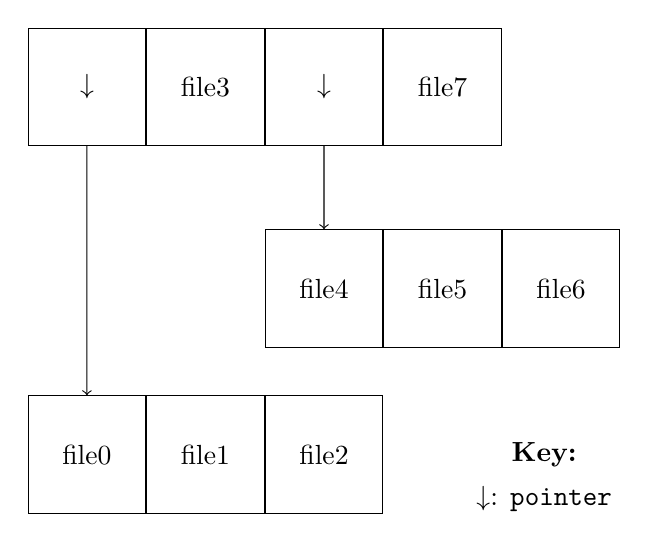
\begin{tikzpicture}[scale=1, square/.style={regular polygon,regular polygon sides=4, minimum width=6em} , x=1cm, y=1cm]
				\node [square,draw] (ptr0) {$\downarrow$};
				\node [square,draw, right=0cm of ptr0] (file3) {file3};
				\node [square,draw, right=0cm of file3] (ptr1) {$\downarrow$};
				\node [square,draw, right=0cm of ptr1] (file7) {file7};
				
				\node [square,draw, below=9em of ptr0] (file0) {file0};
				\node [square,draw, right=0cm of file0] (file1) {file1};
				\node [square,draw, right=0cm of file1 ] (file2) {file2};
				\path [->] (ptr0) edge (file0);
				
				\node [square,draw, below=3em of ptr1] (file4) {file4};
				\node [square,draw, right=0cm of file4] (file5) {file5};
				\node [square,draw, right=0cm of file5] (file6) {file6};
				\path [->] (ptr1) edge (file4);
				
				% Key
				\node [square,right=0cm of file2] (space) {};
				\node [right=0cm of space] (key) {\textbf{Key:}};
				\node [below=0cm of key] (key1) {$\downarrow$: \texttt{pointer}};
			\end{tikzpicture}
		}
	}
	\caption{Example of tree structure for referenced files within a directory\label{fig:b-tree}.}
\end{figure}
\subsection{Hard-links}
A special case in referencing files are hard-links, which means that multiple directories contain the exact same file, just with a different name. In order to allow for these kinds of entries, each directory containing a hard-link to a file will have an index entry, like the example in Figure \ref{fig:extent_file_indicies}, with the respective name of the hard-link. N.B.: The index and size fields of the index entry will be identical across all directories referencing the given file. To count the number of hard-links files have a further, previously omitted attribute: a hard-link counter called \textit{Reference Count}. Upon creation of a hard-link the reference count will be incremented. Upon deletion of a hard-linked file in a directory the entry will be removed, but the file will only be removed if the reference count is one \cite{inv:NLD:2018} otherwise the afore-mentioned value will be decremented. As files contain a reference to their parent directory and a file-name, NTFS will create multiple attributes for this information with each hard-link having its unique attributes. This ensures that hard-links can be renamed or deleted without conflicts\cite{joscon:HHW:2011}. In this case the reference that is to be removed would be the only one to this file. Further it should be noted that to prevent circles in the MFT structure hard-linking directories is not allowed \cite{inv:NLD:2018} and that due to the hard-link counter being 16-bit\cite{inv:NLD:2018}, at most $65,535$ references can exist to a single file.
\subsection{Bitmap}
In order to be able to store files outside of the MFT, it was discussed that they will be stored into clusters. To avoid overwriting existing data NTFS has to keep track of which clusters are currently in use. and use this information to make sure that no clusters are allocated multiple times. To accomplish this, NTFS keeps a file called \texttt{\$BITMAP}, which, as the name suggests, is a bitmap keeping track of which clusters are in use. So for a given cluster with LCN $l$ the $l$\textsuperscript{th} bit is set to $0$ if the cluster is unsued and otherwise the bit is set to $1$ \cite{B:2017:AJI1}.\\
 In order to speed up the process of deleting a directory, most directory entries in the MFT have an attribute called \texttt{\$BITMAP}. This attribute is not to be confused though with the bitmap file discussed before, as it only contains a list of bitmap indices that are currently in use by the directory, such that upon deletion the file tree will not have to be walked again to accumulate  all clusters that are  to be marked as free again \cite{RUSSINOVICH_ET_AL:2012:WI}. This is attribute is used as otherwise each file in a directory would have to be individually queried to find the clusters that the directory uses.\\
 A potential problem with this approach would be that hard linked file's clusters would be referenced in multiple directories' bitmap attributes and might as cause unwanted deltetion upon deleting one of the parent directories of the hard-linked file. To avoid this kind of unwanted deletion, when hard-linking a file, the indices will be removed from the \texttt{\$BITMAP} attribute of the parent directory and will only be readded once the file is only referenced from a single directory again.

\bibliographystyle{abbrv}
\bibliography{ntfs}
%\footnotesize
\end{document}
